
    \documentclass{standalone}
\usepackage{tkz-fct}
\usepackage{tkz-euclide}
\usepackage{color}
\renewcommand*\familydefault{\sfdefault}
\usepackage{sansmath}
\sansmath
\definecolor{gray75}{gray}{0.75}
\begin{document}
 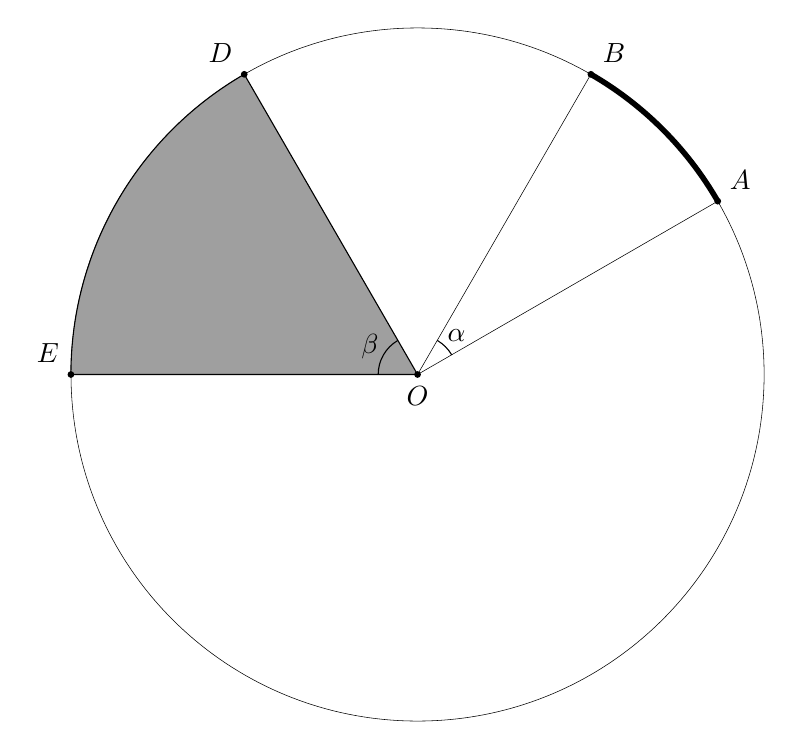
\begin{tikzpicture}[scale=1.1]
   % \tkzInit[xmax=6.0,ymax=6.0,xmin=-6.0 ,ymin=-6.0]
   % \begin{scope}[dashed]
   %   \tkzGrid
   % \end{scope}
   % \tkzDrawX[label={$x$}]
   % \tkzDrawY[label={$y$}]
   % \tkzLabelX
   % \tkzLabelY
   \tkzDefPoints{0/0/O,4/0/P}
   \tkzDrawCircle[color=black](O,P)
   \tkzDefPointBy[rotation= center O angle 30](P)
   \tkzGetPoint{A}
   \tkzDefPointBy[rotation= center O angle 60](P)
   \tkzGetPoint{B}
   \tkzDrawSegment(O,A)
   \tkzDrawSegment(O,B)
   \tkzDrawArc[color=black,line width=2pt](O,A)(B)
   \tkzDefPointBy[rotation= center O angle 120](P)
   \tkzGetPoint{D}
   \tkzDefPointBy[rotation= center O angle 180](P)
   \tkzGetPoint{E}
   \tkzDrawSector[fill=gray!75](O,D)(E)
   \tkzDrawPoints(A,B,D,E,O)
   \tkzPicAngle["$\alpha$",draw=black,
-,angle eccentricity=1.4,
angle radius=0.5cm](A,O,B)
 \tkzPicAngle["$\beta$",draw=black,
-,angle eccentricity=1.4,
angle radius=0.5cm](D,O,E)
\tkzLabelPoints[above right](A,B)
\tkzLabelPoints[above left](D,E)
\tkzLabelPoints[below](O)

\end{tikzpicture}
\end{document}
